\section{652 --- Find Duplicate Subtrees}
Given a binary tree, return all duplicate subtrees. For each kind of duplicate subtrees, you only need to return the root node of any one of them.

Two trees are duplicate if they have the same structure with same node values.

\paragraph{Example 1:}

\begin{flushleft}
\begin{figure}[H]
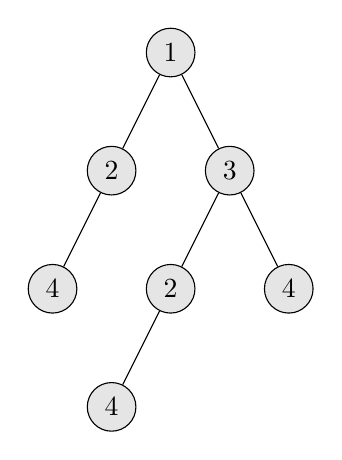
\begin{tikzpicture}
[every node/.style={draw, circle, fill=gray!20!, minimum size=5mm}]
\node{1}
child{node{2} child{node{4}} child[missing]}
child{node{3} child{node{2} child{node{4}} child[missing]} child{node{4}}};
\end{tikzpicture}
\end{figure}

The following are two duplicate subtrees:

\begin{figure}[H]
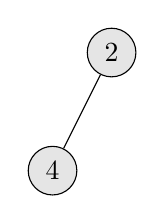
\begin{tikzpicture}
[every node/.style={draw, circle, fill=gray!20!, minimum size=5mm}]
\node{2}
child{node{4}}
child[missing];
\end{tikzpicture}
\end{figure}

\begin{figure}[H]
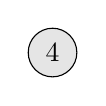
\begin{tikzpicture}
[my/.style={draw, circle, fill=gray!20!, minimum size=5mm}]
\node[my]{4};
\end{tikzpicture}
\end{figure}

Therefore, you need to return above trees' root in the form of a list.
\end{flushleft}

\subsection{Depth First Search}
This approach makes use of DFS to serialize a tree. The result string will be the unique string for this tree. For example, we can serialize the following tree 

\begin{figure}[H]
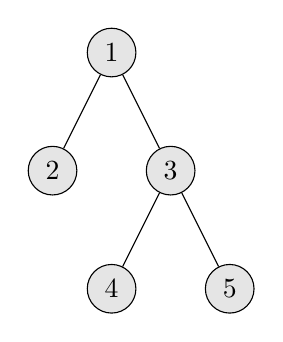
\begin{tikzpicture}
[every node/.style={draw, circle, fill=gray!20!, minimum size=5mm}]
\node{1}
child{node{2}}
child{node{3} child{node{4}} child{node{5}}};
\end{tikzpicture}
\end{figure}

as \lstinline[language=Java, basicstyle=\small\ttfamily, keywordstyle=\bfseries\color{green!40!black}]|1,2,#,#,3,4,#,#,5,#,#|

Thus, we can make use of a hash map to record the count of the same unique strings. When that count is larger than 1, we know we find a duplicate tree. Since we only output one of the root in these trees, we add the node into the output list only when the count is equal to 2.

\subsection{Optimized UUID}
Suppose we have a unique identifier for subtrees: two subtrees are the same if and only if they have the same id.

Then, for a node with left child id of $x$ and right child id of $y$, \lstinline[language=Java, basicstyle=\small\ttfamily, keywordstyle=\bfseries\color{green!40!black}]|(node.val, x, y)| uniquely determines the tree.

In this approach, we make use of two hash maps, say $m_1$ and $m_2$. 
\begin{itemize}
\item $m_1$ record the serialized string of a tree and its related uuid
\item $m_2$ map a tree's uuid to its count.
\end{itemize}

After getting the serialize result of a tree, search its uuid in $m_1$. If this is a new tree, create a new one. Then, we search the uuid in $m_2$. Similar to dfs approach, when this count reaches 2, we add current node into the output list.
